% Demo paper draft for a versioned database testing platform.
% Replace the placeholder authors/institute and the boxed figures as needed.
\documentclass[runningheads]{llncs}
\usepackage[T1]{fontenc}
\usepackage{graphicx}
\usepackage{tikz}
\usetikzlibrary{arrows.meta, positioning, fit, backgrounds, calc}
\usepackage{url}

\begin{document}
%
\title{A Versioned Experimental Platform for Large-Scale Database Benchmarking}
\titlerunning{Versioned Database Testing Platform}
%
\author{Anonymous Authors}
\authorrunning{Anonymous Authors}
%
\institute{Beihang University, Beijing, China}
%
\maketitle
%
\begin{abstract}
Large-scale database testing depends on a stable experimental state, but in practice the workflow is often fragmented across data import, deployment, workload execution, and manual bookkeeping. This fragmentation becomes especially visible when the dataset reaches hundreds of gigabytes, because repeated studies cannot afford to rebuild the same test state from scratch every time. Existing tools each solve only one part of the problem: workload runners execute benchmarks, versioning systems snapshot data, and replay systems preserve traces, but none of them provides a unified experimental lifecycle for repeated database studies. We present a lightweight database testing platform that turns one-time ingest into a reusable snapshot, lets workloads choose between deployment reuse and clean reset, and records each run together with the snapshot, workload, configuration, and Git commit that produced it. The demo walks through import, snapshot archival, deployment reuse, run recovery, and history-based comparison.
\keywords{database testing \and version control \and benchmark \and large-scale data}
\end{abstract}
%
\section{Introduction and Motivation}
Database benchmarking is no longer limited to toy workloads, but the surrounding experiment workflow is still often built ad hoc. A typical study begins with a large data import, then runs a workload, and finally records the Git commit, schema version, or configuration by hand. This is tolerable when the dataset is small, but it becomes fragile when the data reaches hundreds of gigabytes and the system is revised frequently. In that setting, the real research problem is whether repeated executions can start from the same state, remain comparable, and support precise attribution of performance changes.

Existing tools cover only part of this lifecycle, and the missing pieces matter most in large-data settings, where reloading hundreds of gigabytes is often too expensive to repeat for every study. Benchmark frameworks such as BenchBase and OLTPBench can execute workloads against relational DBMSs, but they do not define how a loaded dataset should be frozen into a stable artifact for later studies, so repeated runs may silently begin from different base states. HammerDB provides industrial-strength support for schema building and timed workloads, yet its standard workflow still leaves data preparation, deployment, and repeated execution as separate steps, which forces researchers to decide ad hoc whether to rebuild, reuse, or partially reset a large test environment. Versioning systems such as DVC and lakeFS snapshot large datasets, but they stop before workload execution and therefore cannot capture which workload and configuration produced a result, so a data version alone is not enough to reconstruct the full experiment context. Replay systems such as Oracle Real Application Testing and SQL Server Distributed Replay preserve real traces, but they are tied to specific database ecosystems and do not provide a general experiment-state model for repeated benchmark studies across systems. When the loaded data, deployment, and history records are managed by different tools, large-data experiments can drift into different starting states, restore semantics, and metadata; the resulting measurements can be hard to compare, difficult to reproduce, and ambiguous to attribute.

\noindent\textbf{Contributions.} We design the prototype around three components:
\begin{itemize}
  \item A large-data snapshot pipeline that converts one-time ingest into a reusable experimental state for repeated studies.
  \item A lifecycle-aware workflow that makes deployment reuse or reset depend on workload semantics, so read-only studies can reuse an existing state while update-heavy studies can return to a clean state.
  \item A history-based experiment record that links results to snapshot, workload, configuration, and Git commits, making comparison and regression attribution much easier.
\end{itemize}

\section{Platform Design and Prototype Status}
Figure~\ref{fig:arch} summarizes the platform architecture. The platform is organized around four durable objects. The \emph{snapshot archive} stores the imported dataset once and makes it reusable. The \emph{deployment record} points to the database instance restored from a snapshot. The \emph{workload bundle} captures the benchmark or test script selected for a run. The \emph{run log} stores the outcome together with the snapshot, configuration, and Git commit identifiers. In other words, every experiment is treated as a record that can be replayed or compared later.

The prototype exposes five user-facing actions: \emph{import}, \emph{archive}, \emph{deploy}, \emph{run}, and \emph{compare}. Import loads the raw dataset into the target DBMS. Archive freezes the loaded state into a reusable snapshot. Deploy restores that snapshot into a clean environment when needed. Run executes the selected workload and stores the measured outcome. Compare opens the run history and contrasts two records by snapshot, workload, configuration, or Git commit. This action set is intentionally small so the demo can be explained and remembered quickly.

For each run, the platform records the snapshot identifier, workload identifier, DBMS configuration fingerprint, Git commit, start and end time, and a compact result summary. This is sufficient to answer the two questions that typically matter during database experimentation: what changed, and where did the change come from?

\begin{figure}[t]
\centering
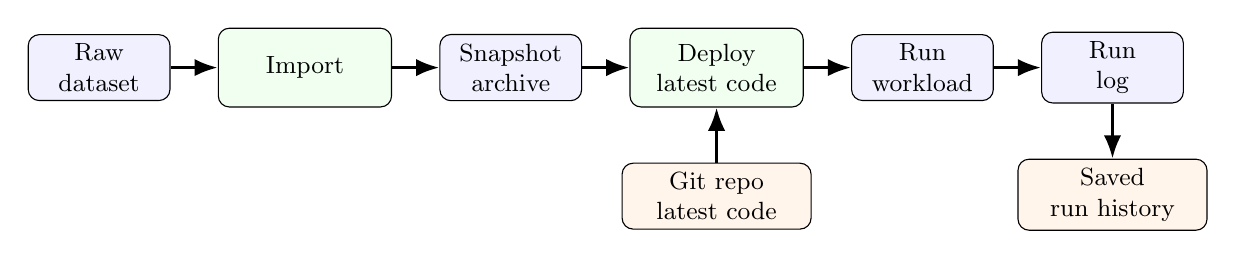
\begin{tikzpicture}[
    font=\small,
    node distance=7mm and 6mm,
    box/.style={draw, rounded corners, align=center, minimum height=8mm, minimum width=18mm, fill=blue!6},
    stage/.style={draw, rounded corners, align=center, minimum height=10mm, minimum width=22mm, fill=green!6},
    note/.style={draw, rounded corners, align=center, minimum height=8mm, minimum width=24mm, fill=orange!8},
    arrow/.style={-Latex, very thick}
]
  \node[box] (raw) {Raw\\dataset};
  \node[stage, right=of raw] (import) {Import};
  \node[box, right=of import] (snap) {Snapshot\\archive};
  \node[stage, right=of snap] (deploy) {Deploy\\latest code};
  \node[box, right=of deploy] (run) {Run\\workload};
  \node[box, right=of run] (log) {Run\\log};

  \node[note, below=of deploy] (git) {Git repo\\latest code};
  \node[note, below=of log] (hist) {Saved\\run history};

  \draw[arrow] (raw) -- (import);
  \draw[arrow] (import) -- (snap);
  \draw[arrow] (snap) -- (deploy);
  \draw[arrow] (deploy) -- (run);
  \draw[arrow] (run) -- (log);
  \draw[arrow] (git.north) -- (deploy.south);
  \draw[arrow] (log.south) -- (hist.north);
\end{tikzpicture}
\caption{Platform architecture. The final version will replace this box with the actual system diagram for import, deployment, Git-backed code refresh, and run history.}
\label{fig:arch}
\end{figure}

This design is deliberately simple. The goal is not to build a new DBMS, but to reduce the overhead of repeated experiments. If a dataset is imported once and materialized as a stable snapshot, later benchmark runs can start from that snapshot instead of replaying the ingest step every time. This matters most when several workload variants must run over the same base data.

\section{Demo Walkthrough}
Figure~\ref{fig:workflow} shows the main user journey. The demo is structured around three scenarios, and each one is designed to answer a practical question that a database engineer would ask when trying to reproduce or compare experiments.

\begin{figure}[t]
\centering
\begin{minipage}[t]{0.46\linewidth}
\centering
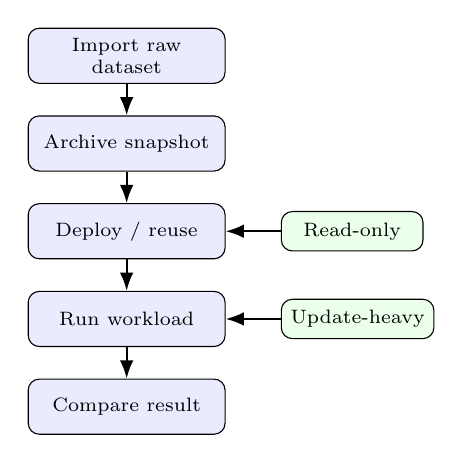
\begin{tikzpicture}[
    font=\scriptsize,
    walkstep/.style={draw, rounded corners, align=center, minimum width=25mm, minimum height=7mm, fill=blue!8},
    smallbox/.style={draw, rounded corners, align=center, minimum width=18mm, minimum height=5mm, fill=green!8},
    arrow/.style={-Latex, thick}
]
  \node[walkstep] (i1) {Import raw\\dataset};
  \node[walkstep, below=4mm of i1] (i2) {Archive snapshot};
  \node[walkstep, below=4mm of i2] (i3) {Deploy / reuse};
  \node[walkstep, below=4mm of i3] (i4) {Run workload};
  \node[walkstep, below=4mm of i4] (i5) {Compare result};

  \draw[arrow] (i1) -- (i2);
  \draw[arrow] (i2) -- (i3);
  \draw[arrow] (i3) -- (i4);
  \draw[arrow] (i4) -- (i5);

  \node[smallbox, right=7mm of i3] (r1) {Read-only};
  \node[smallbox, right=7mm of i4] (r2) {Update-heavy};
  \draw[arrow] (r1.west) -- ++(-3mm,0) |- (i3.east);
  \draw[arrow] (r2.west) -- ++(-3mm,0) |- (i4.east);
\end{tikzpicture}
\par\vspace{1mm}{\scriptsize (a) Import once, deploy many times}
\end{minipage}
\hfill
\begin{minipage}[t]{0.50\linewidth}
\centering
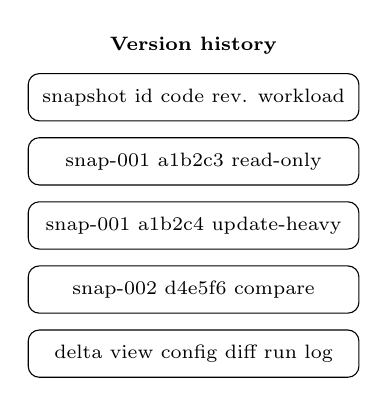
\begin{tikzpicture}[
    font=\scriptsize,
    row/.style={draw, rounded corners, align=left, minimum width=42mm, minimum height=6mm, fill=white},
    arrow/.style={-Latex, thick}
]
  \node[align=left] at (0,0.45) {\textbf{Version history}};
  \node[row, anchor=north] (h1) at (0,0.10) {snapshot id \hfill code rev. \hfill workload};
  \node[row, below=2mm of h1] (h2) {snap-001 \hfill a1b2c3 \hfill read-only};
  \node[row, below=2mm of h2] (h3) {snap-001 \hfill a1b2c4 \hfill update-heavy};
  \node[row, below=2mm of h3] (h4) {snap-002 \hfill d4e5f6 \hfill compare};
  \node[row, below=2mm of h4] (h5) {delta view \hfill config diff \hfill run log};
\end{tikzpicture}
\par\vspace{1mm}{\scriptsize (b) History-based run records}
\end{minipage}
\caption{Demo walkthrough placeholder. Two panels should eventually show the main user journey and the version-history view.}
\label{fig:workflow}
\end{figure}

\subsection{Scenario 1: Import once, test many times}
The first scenario shows how a large dataset is ingested only once. After the ingest finishes, the platform packages the resulting state into a snapshot artifact and registers it in the archive. Multiple benchmark runs can then reuse this snapshot without re-running the full import. This is the core benefit for large datasets: the expensive step is paid only once, while later experiments remain reproducible and directly comparable.

\subsection{Scenario 2: Read-only and update-heavy workloads}
The second scenario compares two workload types. Read-only workloads can be executed directly on a deployed snapshot with no additional recovery step. Update-heavy workloads, on the other hand, are isolated so that the platform can restore the clean snapshot after the run. This makes it possible to test both query-only and modifying workloads without manually rebuilding the database after every experiment. In the demo, this is the part where the audience can see the difference between a reusable deployment and a disposable execution environment.

\subsection{Scenario 3: History-based comparison}
The third scenario highlights the run history. Two runs can be compared side by side using the tags attached to their data, Git commit, and configuration. The demo will show how a user can inspect whether a change comes from the workload, the dataset, the DBMS configuration, or the platform code. This is the main reason we frame the system as a \emph{history-aware} testing platform rather than just a benchmark launcher. The comparison view is also where regression inspection becomes practical, because the user no longer has to guess which component changed between two measurements.

\section{Positioning and Related Work}
Table~\ref{tab:positioning} summarizes the gap we are targeting. The important point is not that the existing systems are weak; rather, each of them is optimized for one slice of the problem. Benchmark runners are good at executing workloads. Versioning tools are good at snapshotting data. Replay tools are good at preserving traces. Our platform links these slices into one lifecycle so that large-data database experiments can be repeated, compared, and rolled back with much less overhead.

\begin{table}[t]
\centering
\small
\caption{Positioning against existing tools.}
\begin{tabular}{p{2.6cm}p{4.4cm}}
\hline
Tool family & Main gap relative to our platform \\
\hline
BenchBase / OLTPBench / HammerDB & Strong at workload execution, but they do not package imported data into reusable snapshots or make deployment a reusable experiment artifact. \\
DVC / lakeFS & Strong at data versioning and rollback, but they do not execute database workloads or compare benchmark runs. \\
Oracle / SQL Server replay & Strong at capture-replay, but they are vendor-centric and not designed as a general benchmark platform. \\
Our platform & Unifies large-data import, snapshot reuse, deployment/test decoupling, and history-based comparison. \\
\hline
\end{tabular}
\label{tab:positioning}
\end{table}

For the demo presentation, we will emphasize two concrete views: the platform dashboard that lists snapshots, deployments, and experiment runs, and the version history view that makes it easy to inspect performance changes. This is the part most useful to users who currently spend too much time on data preparation rather than on the experiment itself. The related-work section can stay short, because the demo value comes mainly from the workflow and the prototype.

\section{Conclusion}
We proposed a lightweight versioned experimental platform for large-scale database benchmarking. The platform is intentionally focused on the experiment lifecycle: import once, package as a snapshot, deploy on demand, run workloads, and compare by history. The demo shows why such a platform is useful even in a mature relational database ecosystem: mature DBMSs still leave users with repeated imports, ad hoc deployment, and version ambiguity. In the final version, we will replace the placeholder figures with the actual architecture diagram, workflow screenshot, and history view. The key point is simple: the platform makes repeat work visible, reusable, and easier to compare after one walkthrough.

\begin{thebibliography}{8}
\bibitem{sqalpel}
M.~L.~Kersten, P.~Koutsourakis, S.~Manegold, and Y.~Zhang:
SQALPEL: A database performance platform. CIDR demo paper (2019).

\bibitem{benchbase}
BenchBase project homepage, \url{https://github.com/cmu-db/benchbase}, last accessed 2026/04/19.

\bibitem{oltpbench}
D.~E.~Difallah, A.~Pavlo, C.~Curino, and P.~Cudr\'{e}-Mauroux:
OLTP-Bench: An extensible testbed for benchmarking relational databases.
PVLDB \textbf{7}(4), 277--288 (2013).

\bibitem{hammerdb}
HammerDB documentation, \url{https://www.hammerdb.com/docs4.11/index.html}, last accessed 2026/04/19.

\bibitem{dvc}
DVC documentation: Versioning data and models,
\url{https://doc.dvc.org/example-scenarios/versioning-data-and-models}, last accessed 2026/04/19.

\bibitem{lakefs}
lakeFS homepage, \url{https://lakefs.io/}, last accessed 2026/04/19.

\bibitem{oracle_replay}
Oracle Real Application Testing documentation,
\url{https://docs.oracle.com/en-us/iaas/autonomous-database-serverless/doc/autonomous-real-application-testing.html}, last accessed 2026/04/19.

\bibitem{sqlserver_replay}
Microsoft SQL Server Distributed Replay overview,
\url{https://learn.microsoft.com/en-us/sql/tools/distributed-replay/sql-server-distributed-replay?view=sql-server-ver17}, last accessed 2026/04/19.
\end{thebibliography}
\end{document}
